
% Inbuilt themes in beamer
\documentclass[aspectratio=169]{beamer}
\usepackage{graphicx}
% Theme choice:
\usetheme{CambridgeUS}

% Title page details: 
\title{Econometrics Discussion Section 2: nonlinear methods} 
\author{John Green}
\date{Spring 2024}


\begin{document}

% Title page
\begin{frame}
    \titlepage 
\end{frame}

% Outline frame
\begin{frame}{Linearity assumption}
    \begin{itemize}
        \item We talk a lot about the OLS assumptions: conditional mean 0 of the error, finite 4th moments, no multicolinearity \dots
        \item Lurking under the hood: assumption the relationship is linear
        \item This is a very strong assumption: think about relationship between earnings and wages
        \item So we may try to relax the assumption of linearity and estimate a more flexible form; but we will focus on models which still fit into the framework of OLS
    \end{itemize}
\end{frame}

\begin{frame}{Polynomial function}
    \begin{itemize}
        \item If relationship between $Y$ and $X$ is not linear, we can try to approximate it by adding polynomials of $X$ into the regression: 
        \begin{itemize}
            \item $Y = \beta_0 + \beta_1 X + \beta_2 X^2 + \dots + \beta_3 X^n + u$
        \end{itemize}
        \item OLS works the same way! Just with new variables which are powers of $X$
        \item Difficult to interpret coefficients
        \item Question: How many factors should we had?
    \end{itemize}
\end{frame}

\begin{frame}{Log approximation}
    \begin{itemize}
        \item To a first approximation, $\log(1+x) \approx x$ for small $x$ (though be careful)
        \begin{itemize}
            \item This means we can think about a change in $\log(x)$ as a percentage change in $x$
        \end{itemize}
        \item Different ways to introduce logs into $Y=X\beta + u$. How should we interpret:
        \begin{itemize}
            \item log-linear
            \item linear-log
            \item log-log
        \end{itemize}
    \end{itemize}
\end{frame}

\begin{frame}{Log approximation}
    \begin{itemize}
        \item To a first approximation, $\log(1+x) \approx x$ for small $x$ (though be careful)
        \begin{itemize}
            \item This means we can think about a change in $\log(x)$ as a percentage change in $x$
        \end{itemize}
        \item Different ways to introduce logs into $Y=X\beta + u$. How should we interpret:
        \begin{itemize}
            \item \textbf{log-linear}: a change of $z$ in $X$ is associated with a $\beta z \%$ change in $Y$
            \item \textbf{linear-log}: a change of $z\%$ in $X$ is associated with a $\beta .0z \%$ change in $Y$
            \item \textbf{log-log}: a change of $z\%$ in $X$ is associated with a $\beta z \%$ change in $Y$
        \end{itemize}
        \item Other (actual) nonlinear forms are possible too
    \end{itemize}
\end{frame}

% \begin{frame}
%     \centering
%     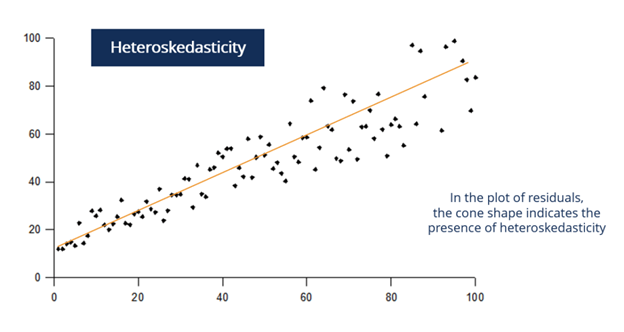
\includegraphics[width = .75\textwidth,keepaspectratio]{./figs/heteroskedasticity.png}
% \end{frame}


\end{document}